\batchmode
\documentclass{book}
\usepackage[letterpaper,top=2.5cm,bottom=2.5cm,left=2.5cm,right=2.5cm]{geometry}
\usepackage{makeidx}
\usepackage{natbib}
\usepackage{graphicx}
\usepackage{multicol}
\usepackage{float}
\usepackage{listings}
\usepackage{color}
\usepackage{ifthen}
\usepackage[table]{xcolor}
\usepackage{textcomp}
\usepackage{alltt}
\usepackage{ifpdf}
\ifpdf
\usepackage[pdftex,
            pagebackref=true,
            colorlinks=true,
            linkcolor=blue,
            unicode
           ]{hyperref}
\else
\usepackage[ps2pdf,
            pagebackref=true,
            colorlinks=true,
            linkcolor=blue,
            unicode
           ]{hyperref}
\usepackage{pspicture}
\fi
\usepackage[utf8]{inputenc}
\usepackage{mathptmx}
\usepackage[scaled=.90]{helvet}
\usepackage{courier}
\usepackage{sectsty}
\usepackage[titles]{tocloft}
\usepackage{doxygen}
\lstset{language=C++,inputencoding=utf8,basicstyle=\footnotesize,breaklines=true,breakatwhitespace=true,tabsize=8,numbers=left }
\usepackage{/Users/rprato/Dropbox/Programacion/Maxwell/config/latexextras}
\makeindex
\setcounter{tocdepth}{3}
\renewcommand{\footrulewidth}{0.4pt}
\renewcommand{\familydefault}{\sfdefault}
\hfuzz=15pt
\setlength{\emergencystretch}{15pt}
\hbadness=750
\tolerance=750
\begin{document}
\hypersetup{pageanchor=false,citecolor=blue}
\begin{titlepage}
\vspace*{7cm}
\begin{center}
{\Large E\-F2\-:Peers\-\_\-\-El \\[1ex]\large 0.\-1 }\\
\vspace*{1cm}
{\large Generated by Doxygen 1.8.0}\\
\vspace*{0.5cm}
{\small Sat Apr 28 2012 11:40:53}\\
\end{center}
\end{titlepage}
\clearemptydoublepage
\pagenumbering{roman}
\tableofcontents
\clearemptydoublepage
\pagenumbering{arabic}
\hypersetup{pageanchor=true,citecolor=blue}
\chapter{Desarrolladores E\-F2}
\label{developers}
\hypertarget{developers}{}
\input{developers}
\chapter{Changes in E\-F2\-:Peers\-\_\-\-El Version 0.1}
\label{changelog0_1}
\hypertarget{changelog0_1}{}

\begin{DoxyRefList}
\item[\label{changelog0_1__changelog0_1000001}%
\hypertarget{changelog0_1__changelog0_1000001}{}%
Member \hyperlink{_bases__func___maxwell_8m_ab0c16723c2e03671e047503c65352c26}{Bases\-\_\-func\-\_\-\-Maxwell} (matlabtypesubstitute u, matlabtypesubstitute i, matlabtypesubstitute j, matlabtypesubstitute x)](\hyperlink{developers_rapt}{Ricardo Prato}, 2012-\/04-\/16)
\end{DoxyRefList}
\chapter{Class Index}
\section{Class Hierarchy}
This inheritance list is sorted roughly, but not completely, alphabetically\-:\begin{DoxyCompactList}
\item \contentsline{section}{cell}{\pageref{a00002}}{}
\item \contentsline{section}{char}{\pageref{a00003}}{}
\item \contentsline{section}{colvec}{\pageref{a00004}}{}
\item \contentsline{section}{double}{\pageref{a00005}}{}
\item \contentsline{section}{function\-\_\-handle}{\pageref{a00006}}{}
\item \contentsline{section}{handle}{\pageref{a00007}}{}
\item \contentsline{section}{integer}{\pageref{a00008}}{}
\item \contentsline{section}{logical}{\pageref{a00009}}{}
\item \contentsline{section}{matrix}{\pageref{a00010}}{}
\begin{DoxyCompactList}
\item \contentsline{section}{sparsematrix}{\pageref{a00012}}{}
\end{DoxyCompactList}
\item \contentsline{section}{rowvec}{\pageref{a00011}}{}
\item \contentsline{section}{struct}{\pageref{a00013}}{}
\item \contentsline{section}{varargin}{\pageref{a00014}}{}
\item \contentsline{section}{varargout}{\pageref{a00015}}{}
\end{DoxyCompactList}

\chapter{Class Index}
\input{annotated}
\chapter{File Index}
\section{File List}
Here is a list of all files with brief descriptions\-:\begin{DoxyCompactList}
\item\contentsline{section}{\hyperlink{a00016}{class\-\_\-substitutes.\-c} }{\pageref{a00016}}{}
\item\contentsline{section}{\hyperlink{a00017}{developers.\-c} }{\pageref{a00017}}{}
\item\contentsline{section}{\hyperlink{a00018}{dirichlet\-\_\-int.\-m} \\*Calcula la integral total de frontera para problemas no homogeneos \[ \int_{ \partial \Omega} \, n \times \curl{\bds{u}} \cdot \bds{\phi}_j \, \mathrm{d}x \] donde $ \bds{\phi}_i $ es una función base (elementos de Whitney en 2\-D) }{\pageref{a00018}}{}
\item\contentsline{section}{\hyperlink{a00019}{E\-\_\-error3.\-m} \\*Calcula el error (en caso de tener solución exacta) \[ \Vert E-E_h \Vert_{H(curl,\Omega)} \] }{\pageref{a00019}}{}
\item\contentsline{section}{\hyperlink{a00020}{Ece.\-m} \\*Calcula el valor de la función exacta (dada en rhs) en el punto xs }{\pageref{a00020}}{}
\item\contentsline{section}{\hyperlink{a00021}{Edgesnum\-\_\-\-Maxwell.\-m} \\*Inicializa la numeración de los lados de la malla provista por malla$\ast$.m y calcula los coeficientes de la funciones bases $ \bds{\phi}_i $ de $ \mathbb{P}_1 $ }{\pageref{a00021}}{}
\item\contentsline{section}{\hyperlink{a00022}{funciones.\-m} \\*String de la función exacta utilizada. Por ejemplo, }{\pageref{a00022}}{}
\item\contentsline{section}{\hyperlink{a00023}{gauss.\-m} \\*Genera los puntos $ x_i $ y los pesos $ w_i $ para una cuadratura Gauss-\/\-Legendre \[ \int_{a}^b W(x) \cdot f(t) dt \approx \sum_{i=1}^{n} w_i \, f(x_i) \] siguiendo lo propuesto en la sección 4.\-6 de \par
 Numerical Recipes\-: The Art of Scientific Computing \par
 Third Edition (2007) \par
 Cambridge University Press \par
 I\-S\-B\-N-\/10\-: 0521880688 }{\pageref{a00023}}{}
\item\contentsline{section}{\hyperlink{a00024}{int\-\_\-time.\-m} \\*Calcula el valor de las integrales \begin{eqnarray*} I_1 =\int_{t_{n-1}}^{t_{n}} (t-t_{m})\cdot t_{n} \cdot g(t) \, dt &\qquad& I_2 =\int_{t_{n-1}}^{t_{n}} (t-t_{m})\cdot t_{n} \cdot g^{\prime}(t) \, dt \\[3mm] I_3 = \int_{t_{n-1}}^{t_{n}} (t-t_{n-1})\cdot t_{n} \cdot g(t) \, dt &\qquad& I_4 = \int_{t_{n-1}}^{t_{n}} (t-t_{n-1})\cdot t_{n} \cdot g^{\prime}(t) \, dt \\[3mm] I_5 = \int_{t_{n-1}}^{t_{n}} (t-t_{n-1})\cdot t_{m} \cdot g(t) \, dt &\qquad& I_6 = \int_{t_{n-1}}^{t_{n}} (t-t_{n-1})\cdot t_{m} \cdot g^{\prime}(t) \, dt \ \end{eqnarray*} }{\pageref{a00024}}{}
\item\contentsline{section}{\hyperlink{a00025}{malla01.\-m} \\*Inicializa la geometria $ [0,1] \times [0,1] $ \par
 }{\pageref{a00025}}{}
\item\contentsline{section}{\hyperlink{a00026}{malla02.\-m} \\*Inicializa la geometria $ [-1,1] \times [-1,1] $ \par
 }{\pageref{a00026}}{}
\item\contentsline{section}{\hyperlink{a00027}{maxwell\-\_\-dgm2.\-m} \\*Programa Principal para la aproximación de soluciones de un problema de Eddy current dependiente del tiempo \begin{eqnarray*} \frac{ \partial \bds{E}}{dt} + \curl{\Big ( \alpha \cdot \curl{E}\Big )} &=& f \mbox{ en $\Omega \times (0,T]$}\\ \bds{E} \times \bds{n} &=& g \mbox{ en $\partial \Omega \times (0,T]$}\\ \bds{E} &=& 0 \mbox{ en $ \Omega \times \{0\}$} \end{eqnarray*} en 2\-D utilizando para la discretización en el tiempo polinomios cuadráticos vía D\-G\-M y para la discrezación del espacio elementos de Whitney }{\pageref{a00027}}{}
\item\contentsline{section}{\hyperlink{a00028}{pt\-\_\-\-J.\-m} \\*Define la función independiente del tiempo asociada al lado derecho \[ f(t,\bds{x})=-\partial_t \bds{J}=\sigma \partial_t \bds{E} + \frac{1}{\mu} \curl{\curl{E}} \] al definir $\bds{E} (t,\bds{x})=g(t) \cdot h(\bds{x})$ }{\pageref{a00028}}{}
\item\contentsline{section}{\hyperlink{a00029}{refine\-R\-G\-B.\-m} \\*Refina la malla provista por malla$\ast$.m utilizando un esquema red-\/green }{\pageref{a00029}}{}
\item\contentsline{section}{\hyperlink{a00030}{rhs\-\_\-\-Maxw.\-m} \\*Acopla la matriz de lado derecho local \[ \int_{\Omega}\,f(x) \bds{\phi}_j \, \mathrm{d}x \] donde $ \bds{\phi}_i $ es una función base (elementos de Whitney en 2\-D) }{\pageref{a00030}}{}
\item\contentsline{section}{\hyperlink{a00031}{shownu.\-m} \\*Grafica la malla, y permite mostrar los elementos, nodos, y lados asociados a la misma }{\pageref{a00031}}{}
\item\contentsline{section}{\hyperlink{a00032}{Stiff\-\_\-\-Maxwell.\-m} \\*Calcula la matriz de rigidez local $ ( \mrom{curl}\,\bds{\phi}_i,\mrom{curl}\,\bds{\phi}_j)_{T_k}$ sobre el elemento $ T_k $ donde $ \bds{\phi}_i $ es una función base (elementos de Whitney en 2\-D) }{\pageref{a00032}}{}
\item\contentsline{section}{\hyperlink{a00033}{Whitney\-\_\-func\-\_\-\-Maxwell.\-m} \\*Calcula el valor en el punto $ \bds{x}$ de la función base $\bds{\phi}^i$ (elementos de Whitney 2\-D) definido por \[ \bds{\phi}^i = \bds{\lambda}_k \cdot \nabla \bds{\lambda}_j - \bds{\lambda}_j \cdot \nabla \bds{\lambda}_k \] donde $ co=[k,\, j] $ }{\pageref{a00033}}{}
\end{DoxyCompactList}

\chapter{Class Documentation}
\hypertarget{classcell}{\section{cell Class Reference}
\label{classcell}\index{cell@{cell}}
}


A Mat\-Lab cell array or matrix.  




\subsection{Detailed Description}
A Mat\-Lab cell array or matrix. 

This class is an artificially created class in doxygen to allow more precise type declarations 

The documentation for this class was generated from the following file\-:\begin{DoxyCompactItemize}
\item 
\hyperlink{class__substitutes_8c}{class\-\_\-substitutes.\-c}\end{DoxyCompactItemize}

\input{classchar}
\hypertarget{classcolvec}{\section{colvec Class Reference}
\label{classcolvec}\index{colvec@{colvec}}
}


A matlab column vector.  




\subsection{Detailed Description}
A matlab column vector. 

This class is an artificially created class in doxygen to allow more precise type declarations 

The documentation for this class was generated from the following file\-:\begin{DoxyCompactItemize}
\item 
\hyperlink{class__substitutes_8c}{class\-\_\-substitutes.\-c}\end{DoxyCompactItemize}

\hypertarget{classdouble}{\section{double Class Reference}
\label{classdouble}\index{double@{double}}
}


A double value.  




\subsection{Detailed Description}
A double value. 

This class is an artificially created class in doxygen to allow more precise type declarations. The Mat\-Lab type associated with this class is double. 

The documentation for this class was generated from the following file\-:\begin{DoxyCompactItemize}
\item 
\hyperlink{class__substitutes_8c}{class\-\_\-substitutes.\-c}\end{DoxyCompactItemize}

\hypertarget{classfunction__handle}{\section{function\-\_\-handle Class Reference}
\label{classfunction__handle}\index{function\-\_\-handle@{function\-\_\-handle}}
}


A Mat\-Lab function handle.  




\subsection{Detailed Description}
A Mat\-Lab function handle. 

This class is an artificially created class in doxygen to allow more precise type declarations 

The documentation for this class was generated from the following file\-:\begin{DoxyCompactItemize}
\item 
\hyperlink{class__substitutes_8c}{class\-\_\-substitutes.\-c}\end{DoxyCompactItemize}

\hypertarget{classhandle}{\section{handle Class Reference}
\label{classhandle}\index{handle@{handle}}
}


Matlab's base handle class (documentation generation substitute)  


\subsection*{Public Attributes}
\begin{DoxyCompactItemize}
\item 
matlabtypesubstitute \hyperlink{classhandle_aa72d46799b8792edbf8acb7349680c15}{addlistener}
\begin{DoxyCompactList}\small\item\em Creates a listener for the specified event and assigns a callback function to execute when the event occurs. \end{DoxyCompactList}\item 
matlabtypesubstitute \hyperlink{classhandle_a8cfc3dab9d3ecc55b0b3449c2c7afd6f}{notify}
\begin{DoxyCompactList}\small\item\em Broadcast a notice that a specific event is occurring on a specified handle object or array of handle objects. \end{DoxyCompactList}\item 
matlabtypesubstitute \hyperlink{classhandle_a1d55d41c7af285b8fe7ab17ed5e176f6}{delete}
\begin{DoxyCompactList}\small\item\em Handle object destructor method that is called when the object's lifecycle ends. \end{DoxyCompactList}\item 
matlabtypesubstitute \hyperlink{classhandle_adedb524cfbdf6a5d946cc57ef6745099}{disp}
\begin{DoxyCompactList}\small\item\em Handle object disp method which is called by the display method. See the M\-A\-T\-L\-A\-B disp function. \end{DoxyCompactList}\item 
matlabtypesubstitute \hyperlink{classhandle_a2e26be32e99b2b98db18bb538638b814}{display}
\begin{DoxyCompactList}\small\item\em Handle object display method called when M\-A\-T\-L\-A\-B software interprets an expression returning a handle object that is not terminated by a semicolon. See the M\-A\-T\-L\-A\-B display function. \end{DoxyCompactList}\item 
matlabtypesubstitute \hyperlink{classhandle_a000398ac90dd973b4618c739e6fd64a9}{findobj}
\begin{DoxyCompactList}\small\item\em Finds objects matching the specified conditions from the input array of handle objects. \end{DoxyCompactList}\item 
matlabtypesubstitute \hyperlink{classhandle_ab4b410e2df940296c9d2563898c951fe}{findprop}
\begin{DoxyCompactList}\small\item\em Returns a meta.\-property objects associated with the specified property name. \end{DoxyCompactList}\item 
matlabtypesubstitute \hyperlink{classhandle_ad9c0557345e68bd933889c28b2a9484b}{fields}
\begin{DoxyCompactList}\small\item\em Returns a cell array of string containing the names of public properties. \end{DoxyCompactList}\item 
matlabtypesubstitute \hyperlink{classhandle_a7086577f3953d4bd9ce17b07c4f6e141}{fieldnames}
\begin{DoxyCompactList}\small\item\em Returns a cell array of string containing the names of public properties. See the M\-A\-T\-L\-A\-B fieldnames function. \end{DoxyCompactList}\item 
matlabtypesubstitute \hyperlink{classhandle_a72617e83dc9643b61ed8af63e5058ccf}{isvalid}
\begin{DoxyCompactList}\small\item\em Returns a logical array in which elements are true if the corresponding elements in the input array are valid handles. This method is Sealed so you cannot override it in a handle subclass. \end{DoxyCompactList}\item 
matlabtypesubstitute \hyperlink{classhandle_a2fb018cd603a5ced1783bfb20c6cce86}{eq}
\begin{DoxyCompactList}\small\item\em Relational functions example. See details for more information. \end{DoxyCompactList}\item 
matlabtypesubstitute \hyperlink{classhandle_acd9b55f206750374c4dfca508cfff084}{transpose}
\begin{DoxyCompactList}\small\item\em Transposes the elements of the handle object array. \end{DoxyCompactList}\item 
matlabtypesubstitute \hyperlink{classhandle_a6dc9f59313af54f392d8e273d71ace7b}{permute}
\begin{DoxyCompactList}\small\item\em Rearranges the dimensions of the handle object array. See the M\-A\-T\-L\-A\-B permute function. \end{DoxyCompactList}\item 
matlabtypesubstitute \hyperlink{classhandle_acef58ae5e52255411835a4fcaf2edd49}{reshape}
\begin{DoxyCompactList}\small\item\em hanges the dimensions of the handle object array to the specified dimensions. See the M\-A\-T\-L\-A\-B reshape function. \end{DoxyCompactList}\item 
matlabtypesubstitute \hyperlink{classhandle_ad11b0be4c173a9d31122c1298eb96a97}{sort}
\begin{DoxyCompactList}\small\item\em ort the handle objects in any array in ascending or descending order. \end{DoxyCompactList}\end{DoxyCompactItemize}


\subsection{Detailed Description}
Matlab's base handle class (documentation generation substitute) 

\begin{DoxyVerb}          As doxygen does not know the class "handle" from itself, many classes do not get rendered within the documentation and the correct root class is not even displayed.
          This workaround guarantees a correct (also graphical) representation of the class hierarchy.\end{DoxyVerb}
 Note here that by having the type handle it could also mean to have a vector or matrix of handles. 

\subsection{Member Data Documentation}
\hypertarget{classhandle_aa72d46799b8792edbf8acb7349680c15}{\index{handle@{handle}!addlistener@{addlistener}}
\index{addlistener@{addlistener}!handle@{handle}}
\subsubsection[{addlistener}]{\setlength{\rightskip}{0pt plus 5cm}matlabtypesubstitute {\bf handle\-::addlistener}}}\label{classhandle_aa72d46799b8792edbf8acb7349680c15}


Creates a listener for the specified event and assigns a callback function to execute when the event occurs. 

\begin{DoxySeeAlso}{See also}
\hyperlink{classhandle_a8cfc3dab9d3ecc55b0b3449c2c7afd6f}{notify} 
\end{DoxySeeAlso}
\hypertarget{classhandle_a1d55d41c7af285b8fe7ab17ed5e176f6}{\index{handle@{handle}!delete@{delete}}
\index{delete@{delete}!handle@{handle}}
\subsubsection[{delete}]{\setlength{\rightskip}{0pt plus 5cm}matlabtypesubstitute {\bf handle\-::delete}}}\label{classhandle_a1d55d41c7af285b8fe7ab17ed5e176f6}


Handle object destructor method that is called when the object's lifecycle ends. 

\hypertarget{classhandle_adedb524cfbdf6a5d946cc57ef6745099}{\index{handle@{handle}!disp@{disp}}
\index{disp@{disp}!handle@{handle}}
\subsubsection[{disp}]{\setlength{\rightskip}{0pt plus 5cm}matlabtypesubstitute {\bf handle\-::disp}}}\label{classhandle_adedb524cfbdf6a5d946cc57ef6745099}


Handle object disp method which is called by the display method. See the M\-A\-T\-L\-A\-B disp function. 

\hypertarget{classhandle_a2e26be32e99b2b98db18bb538638b814}{\index{handle@{handle}!display@{display}}
\index{display@{display}!handle@{handle}}
\subsubsection[{display}]{\setlength{\rightskip}{0pt plus 5cm}matlabtypesubstitute {\bf handle\-::display}}}\label{classhandle_a2e26be32e99b2b98db18bb538638b814}


Handle object display method called when M\-A\-T\-L\-A\-B software interprets an expression returning a handle object that is not terminated by a semicolon. See the M\-A\-T\-L\-A\-B display function. 

\hypertarget{classhandle_a2fb018cd603a5ced1783bfb20c6cce86}{\index{handle@{handle}!eq@{eq}}
\index{eq@{eq}!handle@{handle}}
\subsubsection[{eq}]{\setlength{\rightskip}{0pt plus 5cm}matlabtypesubstitute {\bf handle\-::eq}}}\label{classhandle_a2fb018cd603a5ced1783bfb20c6cce86}


Relational functions example. See details for more information. 

\begin{DoxyParagraph}{Other possible relational operators\-:}
-\/ne -\/lt -\/le -\/gt -\/ge
\end{DoxyParagraph}
Relational functions return a logical array of the same size as the pair of input handle object arrays. Comparisons use a number associated with each handle. You can assume that the same two handles will compare as equal and the repeated comparison of any two handles will yield the same result in the same M\-A\-T\-L\-A\-B session. Different handles are always not-\/equal. The order of handles is purely arbitrary, but consistent. \hypertarget{classhandle_a7086577f3953d4bd9ce17b07c4f6e141}{\index{handle@{handle}!fieldnames@{fieldnames}}
\index{fieldnames@{fieldnames}!handle@{handle}}
\subsubsection[{fieldnames}]{\setlength{\rightskip}{0pt plus 5cm}matlabtypesubstitute {\bf handle\-::fieldnames}}}\label{classhandle_a7086577f3953d4bd9ce17b07c4f6e141}


Returns a cell array of string containing the names of public properties. See the M\-A\-T\-L\-A\-B fieldnames function. 

\hypertarget{classhandle_ad9c0557345e68bd933889c28b2a9484b}{\index{handle@{handle}!fields@{fields}}
\index{fields@{fields}!handle@{handle}}
\subsubsection[{fields}]{\setlength{\rightskip}{0pt plus 5cm}matlabtypesubstitute {\bf handle\-::fields}}}\label{classhandle_ad9c0557345e68bd933889c28b2a9484b}


Returns a cell array of string containing the names of public properties. 

\hypertarget{classhandle_a000398ac90dd973b4618c739e6fd64a9}{\index{handle@{handle}!findobj@{findobj}}
\index{findobj@{findobj}!handle@{handle}}
\subsubsection[{findobj}]{\setlength{\rightskip}{0pt plus 5cm}matlabtypesubstitute {\bf handle\-::findobj}}}\label{classhandle_a000398ac90dd973b4618c739e6fd64a9}


Finds objects matching the specified conditions from the input array of handle objects. 

\hypertarget{classhandle_ab4b410e2df940296c9d2563898c951fe}{\index{handle@{handle}!findprop@{findprop}}
\index{findprop@{findprop}!handle@{handle}}
\subsubsection[{findprop}]{\setlength{\rightskip}{0pt plus 5cm}matlabtypesubstitute {\bf handle\-::findprop}}}\label{classhandle_ab4b410e2df940296c9d2563898c951fe}


Returns a meta.\-property objects associated with the specified property name. 

\hypertarget{classhandle_a72617e83dc9643b61ed8af63e5058ccf}{\index{handle@{handle}!isvalid@{isvalid}}
\index{isvalid@{isvalid}!handle@{handle}}
\subsubsection[{isvalid}]{\setlength{\rightskip}{0pt plus 5cm}matlabtypesubstitute {\bf handle\-::isvalid}}}\label{classhandle_a72617e83dc9643b61ed8af63e5058ccf}


Returns a logical array in which elements are true if the corresponding elements in the input array are valid handles. This method is Sealed so you cannot override it in a handle subclass. 

\hypertarget{classhandle_a8cfc3dab9d3ecc55b0b3449c2c7afd6f}{\index{handle@{handle}!notify@{notify}}
\index{notify@{notify}!handle@{handle}}
\subsubsection[{notify}]{\setlength{\rightskip}{0pt plus 5cm}matlabtypesubstitute {\bf handle\-::notify}}}\label{classhandle_a8cfc3dab9d3ecc55b0b3449c2c7afd6f}


Broadcast a notice that a specific event is occurring on a specified handle object or array of handle objects. 

\hypertarget{classhandle_a6dc9f59313af54f392d8e273d71ace7b}{\index{handle@{handle}!permute@{permute}}
\index{permute@{permute}!handle@{handle}}
\subsubsection[{permute}]{\setlength{\rightskip}{0pt plus 5cm}matlabtypesubstitute {\bf handle\-::permute}}}\label{classhandle_a6dc9f59313af54f392d8e273d71ace7b}


Rearranges the dimensions of the handle object array. See the M\-A\-T\-L\-A\-B permute function. 

\hypertarget{classhandle_acef58ae5e52255411835a4fcaf2edd49}{\index{handle@{handle}!reshape@{reshape}}
\index{reshape@{reshape}!handle@{handle}}
\subsubsection[{reshape}]{\setlength{\rightskip}{0pt plus 5cm}matlabtypesubstitute {\bf handle\-::reshape}}}\label{classhandle_acef58ae5e52255411835a4fcaf2edd49}


hanges the dimensions of the handle object array to the specified dimensions. See the M\-A\-T\-L\-A\-B reshape function. 

\hypertarget{classhandle_ad11b0be4c173a9d31122c1298eb96a97}{\index{handle@{handle}!sort@{sort}}
\index{sort@{sort}!handle@{handle}}
\subsubsection[{sort}]{\setlength{\rightskip}{0pt plus 5cm}matlabtypesubstitute {\bf handle\-::sort}}}\label{classhandle_ad11b0be4c173a9d31122c1298eb96a97}


ort the handle objects in any array in ascending or descending order. 

The order of handles is purely arbitrary, but reproducible in a given M\-A\-T\-L\-A\-B session. See the M\-A\-T\-L\-A\-B sort function. \hypertarget{classhandle_acd9b55f206750374c4dfca508cfff084}{\index{handle@{handle}!transpose@{transpose}}
\index{transpose@{transpose}!handle@{handle}}
\subsubsection[{transpose}]{\setlength{\rightskip}{0pt plus 5cm}matlabtypesubstitute {\bf handle\-::transpose}}}\label{classhandle_acd9b55f206750374c4dfca508cfff084}


Transposes the elements of the handle object array. 



The documentation for this class was generated from the following file\-:\begin{DoxyCompactItemize}
\item 
\hyperlink{class__substitutes_8c}{class\-\_\-substitutes.\-c}\end{DoxyCompactItemize}

\hypertarget{classinteger}{\section{integer Class Reference}
\label{classinteger}\index{integer@{integer}}
}


An integer value.  




\subsection{Detailed Description}
An integer value. 

This class is an artificially created class in doxygen to allow more precise type declarations. Matlab types associated with this class are all int-\/types (int8, uint8 etc). 

The documentation for this class was generated from the following file\-:\begin{DoxyCompactItemize}
\item 
\hyperlink{class__substitutes_8c}{class\-\_\-substitutes.\-c}\end{DoxyCompactItemize}

\hypertarget{classlogical}{\section{logical Class Reference}
\label{classlogical}\index{logical@{logical}}
}


A boolean value.  




\subsection{Detailed Description}
A boolean value. 

This class can be seen as synonym for boolean values/flags used inside classes. In order to stick with matlab conventions/datatypes, this class was named logical instead of bool or boolean.

This class is an artificially created class in doxygen to allow more precise type declarations 

The documentation for this class was generated from the following file\-:\begin{DoxyCompactItemize}
\item 
\hyperlink{class__substitutes_8c}{class\-\_\-substitutes.\-c}\end{DoxyCompactItemize}

\hypertarget{classmatrix}{\section{matrix Class Reference}
\label{classmatrix}\index{matrix@{matrix}}
}


A matlab matrix.  




Inheritance diagram for matrix\-:\nopagebreak
\begin{figure}[H]
\begin{center}
\leavevmode
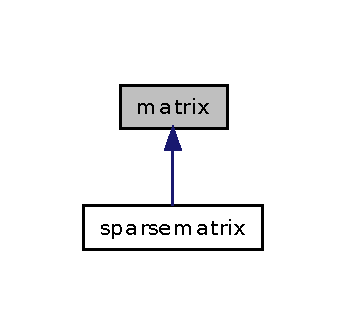
\includegraphics[width=166pt]{classmatrix__inherit__graph}
\end{center}
\end{figure}


\subsection{Detailed Description}
A matlab matrix. 

This class is an artificially created class in doxygen to allow more precise type declarations 

The documentation for this class was generated from the following file\-:\begin{DoxyCompactItemize}
\item 
\hyperlink{class__substitutes_8c}{class\-\_\-substitutes.\-c}\end{DoxyCompactItemize}

\hypertarget{classrowvec}{\section{rowvec Class Reference}
\label{classrowvec}\index{rowvec@{rowvec}}
}


A matlab row vector.  




\subsection{Detailed Description}
A matlab row vector. 

This class is an artificially created class in doxygen to allow more precise type declarations 

The documentation for this class was generated from the following file\-:\begin{DoxyCompactItemize}
\item 
\hyperlink{class__substitutes_8c}{class\-\_\-substitutes.\-c}\end{DoxyCompactItemize}

\hypertarget{classsparsematrix}{\section{sparsematrix Class Reference}
\label{classsparsematrix}\index{sparsematrix@{sparsematrix}}
}


A matlab sparse matrix.  




Inheritance diagram for sparsematrix\-:\nopagebreak
\begin{figure}[H]
\begin{center}
\leavevmode
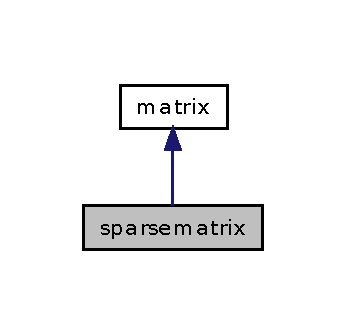
\includegraphics[width=166pt]{classsparsematrix__inherit__graph}
\end{center}
\end{figure}


Collaboration diagram for sparsematrix\-:\nopagebreak
\begin{figure}[H]
\begin{center}
\leavevmode
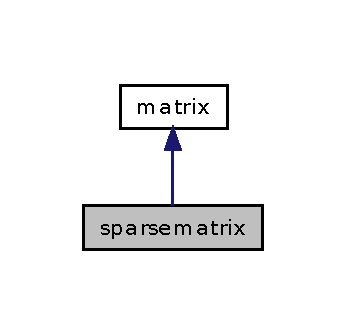
\includegraphics[width=166pt]{classsparsematrix__coll__graph}
\end{center}
\end{figure}


\subsection{Detailed Description}
A matlab sparse matrix. 

This class is an artificially created class in doxygen to allow more precise type declarations 

The documentation for this class was generated from the following file\-:\begin{DoxyCompactItemize}
\item 
\hyperlink{class__substitutes_8c}{class\-\_\-substitutes.\-c}\end{DoxyCompactItemize}

\hypertarget{classstruct}{\section{struct Class Reference}
\label{classstruct}\index{struct@{struct}}
}


A Mat\-Lab struct.  




\subsection{Detailed Description}
A Mat\-Lab struct. 

\begin{DoxyParagraph}{Generated fields of u\-:}

\end{DoxyParagraph}
This class is an artificially created class in doxygen to allow more precise type declarations 

The documentation for this class was generated from the following file\-:\begin{DoxyCompactItemize}
\item 
\hyperlink{maxwell__dgm2_8m}{maxwell\-\_\-dgm2.\-m}\end{DoxyCompactItemize}

\hypertarget{classvarargin}{\section{varargin Class Reference}
\label{classvarargin}\index{varargin@{varargin}}
}


A variable number of input arguments.  




\subsection{Detailed Description}
A variable number of input arguments. 

This class is an artificially created class in doxygen to allow more precise type declarations.

For more information about the varargin argument see the \href{http://www.mathworks.de/help/techdoc/ref/varargin.html}{\tt Mat\-Lab documentation on varargin}. 

The documentation for this class was generated from the following file\-:\begin{DoxyCompactItemize}
\item 
\hyperlink{class__substitutes_8c}{class\-\_\-substitutes.\-c}\end{DoxyCompactItemize}

\hypertarget{classvarargout}{\section{varargout Class Reference}
\label{classvarargout}\index{varargout@{varargout}}
}


A variable number of output arguments.  




\subsection{Detailed Description}
A variable number of output arguments. 

This class is an artificially created class in doxygen to allow more precise type declarations.

For more information about the varargout argument see the \href{http://www.mathworks.de/help/techdoc/ref/varargout.html}{\tt Mat\-Lab documentation on varargout}. 

The documentation for this class was generated from the following file\-:\begin{DoxyCompactItemize}
\item 
\hyperlink{class__substitutes_8c}{class\-\_\-substitutes.\-c}\end{DoxyCompactItemize}

\chapter{File Documentation}
\hypertarget{auxiliar_8m}{\section{auxiliar.\-m File Reference}
\label{auxiliar_8m}\index{auxiliar.\-m@{auxiliar.\-m}}
}
\subsection*{Functions}
\begin{DoxyCompactItemize}
\item 
noret\-::substitute \hyperlink{auxiliar_8m_a9d524ea81d5a1d09d0d75e196fd561da}{auxiliar} ()
\end{DoxyCompactItemize}


\subsection{Function Documentation}
\hypertarget{auxiliar_8m_a9d524ea81d5a1d09d0d75e196fd561da}{\index{auxiliar.\-m@{auxiliar.\-m}!auxiliar@{auxiliar}}
\index{auxiliar@{auxiliar}!auxiliar.m@{auxiliar.\-m}}
\subsubsection[{auxiliar}]{\setlength{\rightskip}{0pt plus 5cm}noret\-::substitute {\bf auxiliar} (
\begin{DoxyParamCaption}
{}
\end{DoxyParamCaption}
)}}\label{auxiliar_8m_a9d524ea81d5a1d09d0d75e196fd561da}

\input{_bases__func___maxwell_8m}
\hypertarget{carst__basftn_8m}{\section{carst\-\_\-basftn.\-m File Reference}
\label{carst__basftn_8m}\index{carst\-\_\-basftn.\-m@{carst\-\_\-basftn.\-m}}
}
\subsection*{Functions}
\begin{DoxyCompactItemize}
\item 
noret\-::substitute \hyperlink{carst__basftn_8m_a8072af7f4fff9b98a37634accbfd27ef}{carst\-\_\-basftn} (matlabtypesubstitute u, matlabtypesubstitute ik, matlabtypesubstitute jk)
\item 
mlhs\-Inner\-Subst\\*
$<$ matlabtypesubstitute, True $>$ \hyperlink{carst__basftn_8m_a4f1f63ed38df896ad6fc00d3c0ced1e9}{mtoc\-\_\-subst\-\_\-carst\-\_\-basftn\-\_\-m\-\_\-tsbus\-\_\-cotm\-\_\-test\-\_\-line} (matlabtypesubstitute P, matlabtypesubstitute P1, matlabtypesubstitute P2)
\end{DoxyCompactItemize}


\subsection{Function Documentation}
\hypertarget{carst__basftn_8m_a8072af7f4fff9b98a37634accbfd27ef}{\index{carst\-\_\-basftn.\-m@{carst\-\_\-basftn.\-m}!carst\-\_\-basftn@{carst\-\_\-basftn}}
\index{carst\-\_\-basftn@{carst\-\_\-basftn}!carst_basftn.m@{carst\-\_\-basftn.\-m}}
\subsubsection[{carst\-\_\-basftn}]{\setlength{\rightskip}{0pt plus 5cm}noret\-::substitute {\bf carst\-\_\-basftn} (
\begin{DoxyParamCaption}
\item[{matlabtypesubstitute}]{u, }
\item[{matlabtypesubstitute}]{ik, }
\item[{matlabtypesubstitute}]{jk}
\end{DoxyParamCaption}
)}}\label{carst__basftn_8m_a8072af7f4fff9b98a37634accbfd27ef}
\hypertarget{carst__basftn_8m_a4f1f63ed38df896ad6fc00d3c0ced1e9}{\index{carst\-\_\-basftn.\-m@{carst\-\_\-basftn.\-m}!mtoc\-\_\-subst\-\_\-carst\-\_\-basftn\-\_\-m\-\_\-tsbus\-\_\-cotm\-\_\-test\-\_\-line@{mtoc\-\_\-subst\-\_\-carst\-\_\-basftn\-\_\-m\-\_\-tsbus\-\_\-cotm\-\_\-test\-\_\-line}}
\index{mtoc\-\_\-subst\-\_\-carst\-\_\-basftn\-\_\-m\-\_\-tsbus\-\_\-cotm\-\_\-test\-\_\-line@{mtoc\-\_\-subst\-\_\-carst\-\_\-basftn\-\_\-m\-\_\-tsbus\-\_\-cotm\-\_\-test\-\_\-line}!carst_basftn.m@{carst\-\_\-basftn.\-m}}
\subsubsection[{mtoc\-\_\-subst\-\_\-carst\-\_\-basftn\-\_\-m\-\_\-tsbus\-\_\-cotm\-\_\-test\-\_\-line}]{\setlength{\rightskip}{0pt plus 5cm}mlhs\-Inner\-Subst$<$matlabtypesubstitute,True$>$ {\bf mtoc\-\_\-subst\-\_\-carst\-\_\-basftn\-\_\-m\-\_\-tsbus\-\_\-cotm\-\_\-test\-\_\-line} (
\begin{DoxyParamCaption}
\item[{matlabtypesubstitute}]{P, }
\item[{matlabtypesubstitute}]{P1, }
\item[{matlabtypesubstitute}]{P2}
\end{DoxyParamCaption}
)}}\label{carst__basftn_8m_a4f1f63ed38df896ad6fc00d3c0ced1e9}

\hypertarget{class__substitutes_8c}{\section{class\-\_\-substitutes.\-c File Reference}
\label{class__substitutes_8c}\index{class\-\_\-substitutes.\-c@{class\-\_\-substitutes.\-c}}
}
\subsection*{Classes}
\begin{DoxyCompactItemize}
\item 
class \hyperlink{classmatrix}{matrix}
\begin{DoxyCompactList}\small\item\em A matlab matrix. \end{DoxyCompactList}\item 
class \hyperlink{classsparsematrix}{sparsematrix}
\begin{DoxyCompactList}\small\item\em A matlab sparse matrix. \end{DoxyCompactList}\item 
class \hyperlink{classhandle}{handle}
\begin{DoxyCompactList}\small\item\em Matlab's base handle class (documentation generation substitute) \end{DoxyCompactList}\end{DoxyCompactItemize}

\hypertarget{developers_8c}{\section{developers.\-c File Reference}
\label{developers_8c}\index{developers.\-c@{developers.\-c}}
}

\hypertarget{_edgesnum___maxwell_8m}{\section{Edgesnum\-\_\-\-Maxwell.\-m File Reference}
\label{_edgesnum___maxwell_8m}\index{Edgesnum\-\_\-\-Maxwell.\-m@{Edgesnum\-\_\-\-Maxwell.\-m}}
}


Inicializa la numeración de los lados de la malla provista por malla$\ast$.m y calcula los coeficientes de la funciones bases $ \bds{\phi}_i $ de $ \mathbb{P}_1 $.  


\subsection*{Functions}
\begin{DoxyCompactItemize}
\item 
mlhs\-Inner\-Subst\\*
$<$ matlabtypesubstitute, u $>$ \hyperlink{_edgesnum___maxwell_8m_a180f38df86468ad73551f258f9debbfe}{Edgesnum\-\_\-\-Maxwell} (matlabtypesubstitute u)
\begin{DoxyCompactList}\small\item\em Inicializa la numeración de los lados de la malla provista por malla$\ast$.m y calcula los coeficientes de la funciones bases $ \bds{\phi}_i $ de $ \mathbb{P}_1 $. \end{DoxyCompactList}\end{DoxyCompactItemize}


\subsection{Detailed Description}
Inicializa la numeración de los lados de la malla provista por malla$\ast$.m y calcula los coeficientes de la funciones bases $ \bds{\phi}_i $ de $ \mathbb{P}_1 $. 

\subsection{Function Documentation}
\hypertarget{_edgesnum___maxwell_8m_a180f38df86468ad73551f258f9debbfe}{\index{Edgesnum\-\_\-\-Maxwell.\-m@{Edgesnum\-\_\-\-Maxwell.\-m}!Edgesnum\-\_\-\-Maxwell@{Edgesnum\-\_\-\-Maxwell}}
\index{Edgesnum\-\_\-\-Maxwell@{Edgesnum\-\_\-\-Maxwell}!Edgesnum_Maxwell.m@{Edgesnum\-\_\-\-Maxwell.\-m}}
\subsubsection[{Edgesnum\-\_\-\-Maxwell}]{\setlength{\rightskip}{0pt plus 5cm}mlhs\-Inner\-Subst$<$ matlabtypesubstitute, u $>$ {\bf Edgesnum\-\_\-\-Maxwell} (
\begin{DoxyParamCaption}
\item[{matlabtypesubstitute}]{u}
\end{DoxyParamCaption}
)}}\label{_edgesnum___maxwell_8m_a180f38df86468ad73551f258f9debbfe}


Inicializa la numeración de los lados de la malla provista por malla$\ast$.m y calcula los coeficientes de la funciones bases $ \bds{\phi}_i $ de $ \mathbb{P}_1 $. 




\begin{DoxyParams}{Parameters}
{\em u} & Estructura que contiene la malla y condiciones de frontera.\\
\hline
\end{DoxyParams}

\begin{DoxyRetVals}{Return values}
{\em u} & Estructura que contiene la malla y condiciones de frontera.\\
\hline
\end{DoxyRetVals}
\begin{DoxyParagraph}{Required fields of u\-:}

\end{DoxyParagraph}
\begin{DoxyParagraph}{Generated fields of u\-:}
\begin{DoxyItemize}
\item {\ttfamily u.\-intnodes~---~} Matriz de orden (No. lados interiores) x 5. Contiene\-: 
\begin{DoxyCode}
 ['Id. nodo1', 'Id. nodo2', 'Id. lado', 'Id. vecino Elem1', 'Id. vecino Elem2' 
      ]
\end{DoxyCode}
 \item {\ttfamily u.\-ed2nod~---~} Matriz de orden (No. lados ) x 2. Contiene\-: 
\begin{DoxyCode}
 ['Id. nodo1', 'Id. nodo2']
\end{DoxyCode}
 \item {\ttfamily u.\-el2ed~---~} Matriz de orden (No. Elementos ) x 3. Contiene\-: 
\begin{DoxyCode}
 ['Id. lado1', 'Id. lado2' 'Id. lado3']
\end{DoxyCode}
 \item {\ttfamily u.\-nel~---~} Entero. Número de elementos . \item {\ttfamily u.\-noedges~---~} Entero. Número de lados. \item {\ttfamily u.\-nointedges~---~} Entero. Número de lados interiores. \item {\ttfamily u.\-noextedges~---~} Entero. Número de lados exteriores . \item {\ttfamily u.\-numnod~---~} Entero. Número de nodos. u.\-freek=Matriz de orden (No. lados libres ) x 1. Contiene\-: 
\begin{DoxyCode}
 ['Id. lado libre ']
\end{DoxyCode}
 u.\-randk=Matriz de orden (No. lados frontera ) x 1. Contiene\-: 
\begin{DoxyCode}
 ['Id. lado frontera']
\end{DoxyCode}
 \item {\ttfamily u.\-dirichlet~---~} Matriz de orden (No. lados dirichlet -\/ordenados-\/ ) x 2. Contiene\-: 
\begin{DoxyCode}
 ['Id. nodo1' 'Id. nodo2']
\end{DoxyCode}
 \item {\ttfamily u.\-alfas~---~} Matriz de orden $ 3 \times 3 \times \mbox{u.nel } $. Calcula la matriz \[ \begin{pmatrix} a_{11} & a_{12} & a_{13} \\ a_{21} & a_{22} & a_{23}\\ a_{31} & a_{32} & a_{33} \end{pmatrix} \] donde $ \bds{\lambda}_i(x,y) = a_{i1}+a_{(i+1)1}x+a_{(i+1)1}y$, define la i-\/esima coordenadas baricentricas asociadas al elemento. \end{DoxyItemize}

\end{DoxyParagraph}
\begin{DoxyAuthor}{Author}
Ricardo Prato 

Catalina Dominguez 
\end{DoxyAuthor}
\begin{DoxyDate}{Date}
2012-\/03-\/20 
\end{DoxyDate}

\hypertarget{funciones_8m}{\section{funciones.\-m File Reference}
\label{funciones_8m}\index{funciones.\-m@{funciones.\-m}}
}


String de la función exacta utilizada. Por ejemplo,.  


\subsection*{Functions}
\begin{DoxyCompactItemize}
\item 
mlhs\-Inner\-Subst\\*
$<$ matlabtypesubstitute, value $>$ \hyperlink{funciones_8m_a0e5b67397a954c71651f4b0fb44bb8fa}{funciones} (matlabtypesubstitute rhs)
\begin{DoxyCompactList}\small\item\em String de la función exacta utilizada. Por ejemplo,. \end{DoxyCompactList}\end{DoxyCompactItemize}


\subsection{Detailed Description}
String de la función exacta utilizada. Por ejemplo,. 
\begin{DoxyCode}
 >> funciones(80)  
\end{DoxyCode}
 \begin{DoxyVerb}     E:=sin(t)*[x*y * (1 - x) * (1 - y)),0]\end{DoxyVerb}
 Parameters\-: rhs\-: Entero. Id. de la función exacta 

\subsection{Function Documentation}
\hypertarget{funciones_8m_a0e5b67397a954c71651f4b0fb44bb8fa}{\index{funciones.\-m@{funciones.\-m}!funciones@{funciones}}
\index{funciones@{funciones}!funciones.m@{funciones.\-m}}
\subsubsection[{funciones}]{\setlength{\rightskip}{0pt plus 5cm}mlhs\-Inner\-Subst$<$ matlabtypesubstitute, value $>$ {\bf funciones} (
\begin{DoxyParamCaption}
\item[{matlabtypesubstitute}]{rhs}
\end{DoxyParamCaption}
)}}\label{funciones_8m_a0e5b67397a954c71651f4b0fb44bb8fa}


String de la función exacta utilizada. Por ejemplo,. 


\begin{DoxyCode}
 >> funciones(80)  
\end{DoxyCode}
 \begin{DoxyVerb}     E:=sin(t)*[x*y * (1 - x) * (1 - y)),0]\end{DoxyVerb}
 Parameters\-: rhs\-: Entero. Id. de la función exacta

\begin{DoxyAuthor}{Author}
Catalina Dominguez 
\end{DoxyAuthor}
\begin{DoxyDate}{Date}
2012-\/03-\/25
\end{DoxyDate}

\begin{DoxyParams}{Parameters}
{\em rhs} & rhs\\
\hline
\end{DoxyParams}

\begin{DoxyRetVals}{Return values}
{\em value} & String . Forma de la solución exacta \\
\hline
\end{DoxyRetVals}

\hypertarget{gauss_8m}{\section{gauss.\-m File Reference}
\label{gauss_8m}\index{gauss.\-m@{gauss.\-m}}
}


Genera los puntos $ x_i $ y los pesos $ w_i $ para una cuadratura Gauss-\/\-Legendre \[ \int_{a}^b W(x) \cdot f(t) dt \approx \sum_{i=1}^{n} w_i \, f(x_i) \] siguiendo lo propuesto en la sección 4.\-6 de \par
 Numerical Recipes\-: The Art of Scientific Computing \par
 Third Edition (2007) \par
 Cambridge University Press \par
 I\-S\-B\-N-\/10\-: 0521880688.  


\subsection*{Functions}
\begin{DoxyCompactItemize}
\item 
mlhs\-Subst$<$ mlhs\-Inner\-Subst\\*
$<$ matlabtypesubstitute, x $>$\\*
,mlhs\-Inner\-Subst\\*
$<$ matlabtypesubstitute, w $>$ $>$ \hyperlink{gauss_8m_a5cac7731040a0693793dfebeeb1bf85b}{gauss} (matlabtypesubstitute n)
\begin{DoxyCompactList}\small\item\em Genera los puntos $ x_i $ y los pesos $ w_i $ para una cuadratura Gauss-\/\-Legendre \[ \int_{a}^b W(x) \cdot f(t) dt \approx \sum_{i=1}^{n} w_i \, f(x_i) \] siguiendo lo propuesto en la sección 4.\-6 de \par
 Numerical Recipes\-: The Art of Scientific Computing \par
 Third Edition (2007) \par
 Cambridge University Press \par
 I\-S\-B\-N-\/10\-: 0521880688. \end{DoxyCompactList}\end{DoxyCompactItemize}


\subsection{Detailed Description}
Genera los puntos $ x_i $ y los pesos $ w_i $ para una cuadratura Gauss-\/\-Legendre \[ \int_{a}^b W(x) \cdot f(t) dt \approx \sum_{i=1}^{n} w_i \, f(x_i) \] siguiendo lo propuesto en la sección 4.\-6 de \par
 Numerical Recipes\-: The Art of Scientific Computing \par
 Third Edition (2007) \par
 Cambridge University Press \par
 I\-S\-B\-N-\/10\-: 0521880688. 

\subsection{Function Documentation}
\hypertarget{gauss_8m_a5cac7731040a0693793dfebeeb1bf85b}{\index{gauss.\-m@{gauss.\-m}!gauss@{gauss}}
\index{gauss@{gauss}!gauss.m@{gauss.\-m}}
\subsubsection[{gauss}]{\setlength{\rightskip}{0pt plus 5cm}mlhs\-Subst$<$ mlhs\-Inner\-Subst$<$ matlabtypesubstitute, x $>$,mlhs\-Inner\-Subst$<$ matlabtypesubstitute, w $>$ $>$ {\bf gauss} (
\begin{DoxyParamCaption}
\item[{matlabtypesubstitute}]{n}
\end{DoxyParamCaption}
)}}\label{gauss_8m_a5cac7731040a0693793dfebeeb1bf85b}


Genera los puntos $ x_i $ y los pesos $ w_i $ para una cuadratura Gauss-\/\-Legendre \[ \int_{a}^b W(x) \cdot f(t) dt \approx \sum_{i=1}^{n} w_i \, f(x_i) \] siguiendo lo propuesto en la sección 4.\-6 de \par
 Numerical Recipes\-: The Art of Scientific Computing \par
 Third Edition (2007) \par
 Cambridge University Press \par
 I\-S\-B\-N-\/10\-: 0521880688. 


\begin{DoxyParams}{Parameters}
{\em n} & número de puntos de cuadratura\\
\hline
\end{DoxyParams}

\begin{DoxyRetVals}{Return values}
{\em x} & Puntos de cuadratura \\
\hline
{\em w} & Pesos Gaussianos \\
\hline
\end{DoxyRetVals}
\begin{DoxyAuthor}{Author}
Ricardo Prato 

Catalina Dominguez 
\end{DoxyAuthor}
\begin{DoxyDate}{Date}
2012-\/03-\/24 
\end{DoxyDate}

\hypertarget{genbasftn_8m}{\section{genbasftn.\-m File Reference}
\label{genbasftn_8m}\index{genbasftn.\-m@{genbasftn.\-m}}
}
\subsection*{Functions}
\begin{DoxyCompactItemize}
\item 
noret\-::substitute \hyperlink{genbasftn_8m_ae0af8b0a0efed26eea68c3c950029c2d}{genbasftn} (matlabtypesubstitute u, matlabtypesubstitute i, matlabtypesubstitute jk)
\end{DoxyCompactItemize}


\subsection{Function Documentation}
\hypertarget{genbasftn_8m_ae0af8b0a0efed26eea68c3c950029c2d}{\index{genbasftn.\-m@{genbasftn.\-m}!genbasftn@{genbasftn}}
\index{genbasftn@{genbasftn}!genbasftn.m@{genbasftn.\-m}}
\subsubsection[{genbasftn}]{\setlength{\rightskip}{0pt plus 5cm}noret\-::substitute {\bf genbasftn} (
\begin{DoxyParamCaption}
\item[{matlabtypesubstitute}]{u, }
\item[{matlabtypesubstitute}]{i, }
\item[{matlabtypesubstitute}]{jk}
\end{DoxyParamCaption}
)}}\label{genbasftn_8m_ae0af8b0a0efed26eea68c3c950029c2d}

\hypertarget{inside__triangle_8m}{\section{inside\-\_\-triangle.\-m File Reference}
\label{inside__triangle_8m}\index{inside\-\_\-triangle.\-m@{inside\-\_\-triangle.\-m}}
}


inside\-\_\-triangle is used to check if a point P is inside the triangle P1\-P2\-P3 or not.  


\subsection*{Functions}
\begin{DoxyCompactItemize}
\item 
mlhs\-Inner\-Subst\\*
$<$ matlabtypesubstitute, True $>$ \hyperlink{inside__triangle_8m_a3cd054bdd41bee0cf4168c190d8d3730}{inside\-\_\-triangle} (matlabtypesubstitute P, matlabtypesubstitute P1, matlabtypesubstitute P2, matlabtypesubstitute P3)
\begin{DoxyCompactList}\small\item\em inside\-\_\-triangle is used to check if a point P is inside the triangle P1\-P2\-P3 or not. \end{DoxyCompactList}\end{DoxyCompactItemize}


\subsection{Detailed Description}
inside\-\_\-triangle is used to check if a point P is inside the triangle P1\-P2\-P3 or not. 

\subsection{Function Documentation}
\hypertarget{inside__triangle_8m_a3cd054bdd41bee0cf4168c190d8d3730}{\index{inside\-\_\-triangle.\-m@{inside\-\_\-triangle.\-m}!inside\-\_\-triangle@{inside\-\_\-triangle}}
\index{inside\-\_\-triangle@{inside\-\_\-triangle}!inside_triangle.m@{inside\-\_\-triangle.\-m}}
\subsubsection[{inside\-\_\-triangle}]{\setlength{\rightskip}{0pt plus 5cm}mlhs\-Inner\-Subst$<$ matlabtypesubstitute, True $>$ {\bf inside\-\_\-triangle} (
\begin{DoxyParamCaption}
\item[{matlabtypesubstitute}]{P, }
\item[{matlabtypesubstitute}]{P1, }
\item[{matlabtypesubstitute}]{P2, }
\item[{matlabtypesubstitute}]{P3}
\end{DoxyParamCaption}
)}}\label{inside__triangle_8m_a3cd054bdd41bee0cf4168c190d8d3730}


inside\-\_\-triangle is used to check if a point P is inside the triangle P1\-P2\-P3 or not. 

Inputs\-: P, P1, P2 and P3 are vectors of length 2 or three of the form \mbox{[}x y z\mbox{]} or \mbox{[}x y\mbox{]}

Output\-: True True=1 =$>$ P is on or inside P1\-P2\-P3 True=0 =$>$ P is outside P1\-P2\-P3

\begin{DoxyParagraph}{Example}
True=inside\-\_\-triangle(\mbox{[}0.\-5 0.\-5\mbox{]},\mbox{[}0 0\mbox{]},\mbox{[}0 2\mbox{]},\mbox{[}2 0\mbox{]});
\end{DoxyParagraph}
The following algorithm is implemented If P is O\-N or I\-N\-S\-I\-D\-E the triangle \begin{DoxyVerb} Area(PP1P2) + Area(PP2P3) + Area(PP3P1) = Area(P1P2P3)\end{DoxyVerb}
 If P is O\-U\-T\-S\-I\-D\-E then, \begin{DoxyVerb} Area(PP1P2) + Area(PP2P3) + Area(PP3P1) > Area(P1P2P3)\end{DoxyVerb}
 \begin{DoxyParagraph}{Area of a triangle can be found using the determinant}
\begin{DoxyVerb}  Area = abs(1/2 * |x1  y1  1| )
                            |x2  y2  1|
                            |x3  y3  1|\end{DoxyVerb}
 
\end{DoxyParagraph}

\begin{DoxyParams}{Parameters}
{\em P} & P \\
\hline
{\em P1} & P1 \\
\hline
{\em P2} & P2 \\
\hline
{\em P3} & P3\\
\hline
\end{DoxyParams}

\begin{DoxyRetVals}{Return values}
{\em True} & True \\
\hline
\end{DoxyRetVals}

\hypertarget{intextnodes_8m}{\section{intextnodes.\-m File Reference}
\label{intextnodes_8m}\index{intextnodes.\-m@{intextnodes.\-m}}
}
\subsection*{Functions}
\begin{DoxyCompactItemize}
\item 
mlhs\-Inner\-Subst\\*
$<$ matlabtypesubstitute, u $>$ \hyperlink{intextnodes_8m_afa3c3242f3cd4d4d74778785352063b1}{intextnodes} (matlabtypesubstitute u)
\item 
mlhs\-Inner\-Subst\\*
$<$ matlabtypesubstitute, alfa $>$ \hyperlink{intextnodes_8m_ac8689c19434fa61d2336e1065ca4dea2}{mtoc\-\_\-subst\-\_\-intextnodes\-\_\-m\-\_\-tsbus\-\_\-cotm\-\_\-inv\-M} (matlabtypesubstitute p, matlabtypesubstitute q, matlabtypesubstitute r)
\end{DoxyCompactItemize}


\subsection{Function Documentation}
\hypertarget{intextnodes_8m_afa3c3242f3cd4d4d74778785352063b1}{\index{intextnodes.\-m@{intextnodes.\-m}!intextnodes@{intextnodes}}
\index{intextnodes@{intextnodes}!intextnodes.m@{intextnodes.\-m}}
\subsubsection[{intextnodes}]{\setlength{\rightskip}{0pt plus 5cm}mlhs\-Inner\-Subst$<$matlabtypesubstitute,u$>$ {\bf intextnodes} (
\begin{DoxyParamCaption}
\item[{matlabtypesubstitute}]{u}
\end{DoxyParamCaption}
)}}\label{intextnodes_8m_afa3c3242f3cd4d4d74778785352063b1}
\hypertarget{intextnodes_8m_ac8689c19434fa61d2336e1065ca4dea2}{\index{intextnodes.\-m@{intextnodes.\-m}!mtoc\-\_\-subst\-\_\-intextnodes\-\_\-m\-\_\-tsbus\-\_\-cotm\-\_\-inv\-M@{mtoc\-\_\-subst\-\_\-intextnodes\-\_\-m\-\_\-tsbus\-\_\-cotm\-\_\-inv\-M}}
\index{mtoc\-\_\-subst\-\_\-intextnodes\-\_\-m\-\_\-tsbus\-\_\-cotm\-\_\-inv\-M@{mtoc\-\_\-subst\-\_\-intextnodes\-\_\-m\-\_\-tsbus\-\_\-cotm\-\_\-inv\-M}!intextnodes.m@{intextnodes.\-m}}
\subsubsection[{mtoc\-\_\-subst\-\_\-intextnodes\-\_\-m\-\_\-tsbus\-\_\-cotm\-\_\-inv\-M}]{\setlength{\rightskip}{0pt plus 5cm}mlhs\-Inner\-Subst$<$matlabtypesubstitute,alfa$>$ {\bf mtoc\-\_\-subst\-\_\-intextnodes\-\_\-m\-\_\-tsbus\-\_\-cotm\-\_\-inv\-M} (
\begin{DoxyParamCaption}
\item[{matlabtypesubstitute}]{p, }
\item[{matlabtypesubstitute}]{q, }
\item[{matlabtypesubstitute}]{r}
\end{DoxyParamCaption}
)}}\label{intextnodes_8m_ac8689c19434fa61d2336e1065ca4dea2}

\hypertarget{main_8m}{\section{main.\-m File Reference}
\label{main_8m}\index{main.\-m@{main.\-m}}
}


fafdfdfsdfsdfs \[ |I_2|=\left| \int_{0}^T \psi(t) \left\{ u(a,t)- \int_{\gamma(t)}^a \frac{d\theta}{k(\theta,t)} \int_{a}^\theta c(\xi)u_t(\xi,t)\,d\xi \right\} dt \right| \]  


\subsection*{Functions}
\begin{DoxyCompactItemize}
\item 
mlhs\-Inner\-Subst\\*
$<$ matlabtypesubstitute, u $>$ \hyperlink{main_8m_a3118aa347aed1173404c5649e9f57edc}{main} (matlabtypesubstitute mode, matlabtypesubstitute rhs, matlabtypesubstitute iter)
\begin{DoxyCompactList}\small\item\em fafdfdfsdfsdfs \[ |I_2|=\left| \int_{0}^T \psi(t) \left\{ u(a,t)- \int_{\gamma(t)}^a \frac{d\theta}{k(\theta,t)} \int_{a}^\theta c(\xi)u_t(\xi,t)\,d\xi \right\} dt \right| \] \end{DoxyCompactList}\end{DoxyCompactItemize}


\subsection{Detailed Description}
fafdfdfsdfsdfs \[ |I_2|=\left| \int_{0}^T \psi(t) \left\{ u(a,t)- \int_{\gamma(t)}^a \frac{d\theta}{k(\theta,t)} \int_{a}^\theta c(\xi)u_t(\xi,t)\,d\xi \right\} dt \right| \] 

\subsection{Function Documentation}
\hypertarget{main_8m_a3118aa347aed1173404c5649e9f57edc}{\index{main.\-m@{main.\-m}!main@{main}}
\index{main@{main}!main.m@{main.\-m}}
\subsubsection[{main}]{\setlength{\rightskip}{0pt plus 5cm}mlhs\-Inner\-Subst$<$ matlabtypesubstitute, u $>$ {\bf main} (
\begin{DoxyParamCaption}
\item[{matlabtypesubstitute}]{mode, }
\item[{matlabtypesubstitute}]{rhs, }
\item[{matlabtypesubstitute}]{iter}
\end{DoxyParamCaption}
)}}\label{main_8m_a3118aa347aed1173404c5649e9f57edc}


fafdfdfsdfsdfs \[ |I_2|=\left| \int_{0}^T \psi(t) \left\{ u(a,t)- \int_{\gamma(t)}^a \frac{d\theta}{k(\theta,t)} \int_{a}^\theta c(\xi)u_t(\xi,t)\,d\xi \right\} dt \right| \] 


\begin{DoxyParams}{Parameters}
{\em mode} & mode \\
\hline
{\em rhs} & rhs \\
\hline
{\em iter} & iter\\
\hline
\end{DoxyParams}

\begin{DoxyRetVals}{Return values}
{\em u} & u \\
\hline
\end{DoxyRetVals}

\hypertarget{malla01_8m}{\section{malla01.\-m File Reference}
\label{malla01_8m}\index{malla01.\-m@{malla01.\-m}}
}


Inicializa la geometria $ [0,1] \times [0,1] $ \par
.  


\subsection*{Functions}
\begin{DoxyCompactItemize}
\item 
mlhs\-Inner\-Subst\\*
$<$ matlabtypesubstitute, u $>$ \hyperlink{malla01_8m_ac07ed38a984c8ec43246d07fd453cd8a}{malla01} (matlabtypesubstitute mode)
\begin{DoxyCompactList}\small\item\em Inicializa la geometria $ [0,1] \times [0,1] $ \par
. \end{DoxyCompactList}\end{DoxyCompactItemize}


\subsection{Detailed Description}
Inicializa la geometria $ [0,1] \times [0,1] $ \par
. 

\subsection{Function Documentation}
\hypertarget{malla01_8m_ac07ed38a984c8ec43246d07fd453cd8a}{\index{malla01.\-m@{malla01.\-m}!malla01@{malla01}}
\index{malla01@{malla01}!malla01.m@{malla01.\-m}}
\subsubsection[{malla01}]{\setlength{\rightskip}{0pt plus 5cm}mlhs\-Inner\-Subst$<$ matlabtypesubstitute, u $>$ {\bf malla01} (
\begin{DoxyParamCaption}
\item[{matlabtypesubstitute}]{mode}
\end{DoxyParamCaption}
)}}\label{malla01_8m_ac07ed38a984c8ec43246d07fd453cd8a}


Inicializa la geometria $ [0,1] \times [0,1] $ \par
. 




\begin{DoxyParams}{Parameters}
{\em mode} & Entero. Determina las condiciones de frontera
\begin{DoxyItemize}
\item mode=1\-: Dirichlet
\item mode $>$ 1\-: Condiciones Mixtas o Neumann
\end{DoxyItemize}\\
\hline
\end{DoxyParams}

\begin{DoxyRetVals}{Return values}
{\em u} & Estructura que contiene la malla y condiciones de frontera.\\
\hline
\end{DoxyRetVals}
\begin{DoxyParagraph}{Generated fields of u\-:}
\begin{DoxyItemize}
\item {\ttfamily u.\-node~---~} Matriz de orden (No. Puntos) x 2. Contiene las coordenadas de los puntos. \item {\ttfamily u.\-pnod~---~} Matriz de orden (No. Elementos) x 3. Contiene los nodos de cada elemento \item {\ttfamily u.\-numnod~---~} Entero. Número de nodos. \item {\ttfamily u.\-Dirich~---~} Matriz de orden (No. lados Dirichlet) x 2. Contiene los nodos de cada elemento de frontera con condición de Dirichlet. \item {\ttfamily u.\-Neumann~---~} Matriz de orden (No. lados Neumann) x 2. Contiene los nodos de cada elemento de frontera con condición de Neumann. \end{DoxyItemize}

\end{DoxyParagraph}
\begin{DoxyAuthor}{Author}
Ricardo Prato 

Catalina Dominguez 
\end{DoxyAuthor}
\begin{DoxyDate}{Date}
2012-\/03-\/20 
\end{DoxyDate}

\hypertarget{provide_geometric_data_8m}{\section{provide\-Geometric\-Data.\-m File Reference}
\label{provide_geometric_data_8m}\index{provide\-Geometric\-Data.\-m@{provide\-Geometric\-Data.\-m}}
}
\subsection*{Functions}
\begin{DoxyCompactItemize}
\item 
mlhs\-Subst$<$ mlhs\-Inner\-Subst\\*
$<$ matlabtypesubstitute, \\*
edge2nodes $>$,mlhs\-Inner\-Subst\\*
$<$ matlabtypesubstitute, \\*
element2edges $>$,mlhs\-Inner\-Subst\\*
$<$ matlabtypesubstitute, \\*
\hyperlink{classvarargout}{varargout} $>$ $>$ \hyperlink{provide_geometric_data_8m_a06424a2b349443e3f5a655b1c36fd0b4}{provide\-Geometric\-Data} (matlabtypesubstitute elements, matlabtypesubstitute \hyperlink{classvarargin}{varargin})
\end{DoxyCompactItemize}


\subsection{Function Documentation}
\hypertarget{provide_geometric_data_8m_a06424a2b349443e3f5a655b1c36fd0b4}{\index{provide\-Geometric\-Data.\-m@{provide\-Geometric\-Data.\-m}!provide\-Geometric\-Data@{provide\-Geometric\-Data}}
\index{provide\-Geometric\-Data@{provide\-Geometric\-Data}!provideGeometricData.m@{provide\-Geometric\-Data.\-m}}
\subsubsection[{provide\-Geometric\-Data}]{\setlength{\rightskip}{0pt plus 5cm}mlhs\-Subst$<$mlhs\-Inner\-Subst$<$matlabtypesubstitute,edge2nodes$>$ ,mlhs\-Inner\-Subst$<$matlabtypesubstitute,element2edges$>$ ,mlhs\-Inner\-Subst$<$matlabtypesubstitute,{\bf varargout}$>$ $>$ {\bf provide\-Geometric\-Data} (
\begin{DoxyParamCaption}
\item[{matlabtypesubstitute}]{elements, }
\item[{matlabtypesubstitute}]{varargin}
\end{DoxyParamCaption}
)}}\label{provide_geometric_data_8m_a06424a2b349443e3f5a655b1c36fd0b4}

\hypertarget{refine_r_g_b_8m}{\section{refine\-R\-G\-B.\-m File Reference}
\label{refine_r_g_b_8m}\index{refine\-R\-G\-B.\-m@{refine\-R\-G\-B.\-m}}
}


Refina la malla provista por malla$\ast$.m utilizando un esquema red-\/green.  


\subsection*{Functions}
\begin{DoxyCompactItemize}
\item 
mlhs\-Subst$<$ mlhs\-Inner\-Subst\\*
$<$ matlabtypesubstitute, \\*
coordenadas $>$,mlhs\-Inner\-Subst\\*
$<$ matlabtypesubstitute, \\*
new\-Elements $>$,mlhs\-Inner\-Subst\\*
$<$ matlabtypesubstitute, \\*
\hyperlink{classvarargout}{varargout} $>$ $>$ \hyperlink{refine_r_g_b_8m_af36e1519bec7348bc4c928967c93800d}{refine\-R\-G\-B} (matlabtypesubstitute coordenadas, matlabtypesubstitute elements, matlabtypesubstitute \hyperlink{classvarargin}{varargin})
\begin{DoxyCompactList}\small\item\em Refina la malla provista por malla$\ast$.m utilizando un esquema red-\/green. \end{DoxyCompactList}\item 
mlhs\-Subst$<$ mlhs\-Inner\-Subst\\*
$<$ matlabtypesubstitute, \\*
edge2nodes $>$,mlhs\-Inner\-Subst\\*
$<$ matlabtypesubstitute, \\*
element2edges $>$,mlhs\-Inner\-Subst\\*
$<$ matlabtypesubstitute, \\*
\hyperlink{classvarargout}{varargout} $>$ $>$ \hyperlink{refine_r_g_b_8m_ab13f3537346ad3e10bb5f966d70ab360}{mtoc\-\_\-subst\-\_\-refine\-R\-G\-B\-\_\-m\-\_\-tsbus\-\_\-cotm\-\_\-\-Geometria} (matlabtypesubstitute elements, matlabtypesubstitute \hyperlink{classvarargin}{varargin})
\end{DoxyCompactItemize}


\subsection{Detailed Description}
Refina la malla provista por malla$\ast$.m utilizando un esquema red-\/green. 

\subsection{Function Documentation}
\hypertarget{refine_r_g_b_8m_ab13f3537346ad3e10bb5f966d70ab360}{\index{refine\-R\-G\-B.\-m@{refine\-R\-G\-B.\-m}!mtoc\-\_\-subst\-\_\-refine\-R\-G\-B\-\_\-m\-\_\-tsbus\-\_\-cotm\-\_\-\-Geometria@{mtoc\-\_\-subst\-\_\-refine\-R\-G\-B\-\_\-m\-\_\-tsbus\-\_\-cotm\-\_\-\-Geometria}}
\index{mtoc\-\_\-subst\-\_\-refine\-R\-G\-B\-\_\-m\-\_\-tsbus\-\_\-cotm\-\_\-\-Geometria@{mtoc\-\_\-subst\-\_\-refine\-R\-G\-B\-\_\-m\-\_\-tsbus\-\_\-cotm\-\_\-\-Geometria}!refineRGB.m@{refine\-R\-G\-B.\-m}}
\subsubsection[{mtoc\-\_\-subst\-\_\-refine\-R\-G\-B\-\_\-m\-\_\-tsbus\-\_\-cotm\-\_\-\-Geometria}]{\setlength{\rightskip}{0pt plus 5cm}mlhs\-Subst$<$mlhs\-Inner\-Subst$<$matlabtypesubstitute,edge2nodes$>$ ,mlhs\-Inner\-Subst$<$matlabtypesubstitute,element2edges$>$ ,mlhs\-Inner\-Subst$<$matlabtypesubstitute,{\bf varargout}$>$ $>$ {\bf mtoc\-\_\-subst\-\_\-refine\-R\-G\-B\-\_\-m\-\_\-tsbus\-\_\-cotm\-\_\-\-Geometria} (
\begin{DoxyParamCaption}
\item[{matlabtypesubstitute}]{elements, }
\item[{matlabtypesubstitute}]{varargin}
\end{DoxyParamCaption}
)}}\label{refine_r_g_b_8m_ab13f3537346ad3e10bb5f966d70ab360}
\hypertarget{refine_r_g_b_8m_af36e1519bec7348bc4c928967c93800d}{\index{refine\-R\-G\-B.\-m@{refine\-R\-G\-B.\-m}!refine\-R\-G\-B@{refine\-R\-G\-B}}
\index{refine\-R\-G\-B@{refine\-R\-G\-B}!refineRGB.m@{refine\-R\-G\-B.\-m}}
\subsubsection[{refine\-R\-G\-B}]{\setlength{\rightskip}{0pt plus 5cm}mlhs\-Subst$<$ mlhs\-Inner\-Subst$<$ matlabtypesubstitute, coordenadas $>$,mlhs\-Inner\-Subst$<$ matlabtypesubstitute, new\-Elements $>$,mlhs\-Inner\-Subst$<$ matlabtypesubstitute, {\bf varargout} $>$ $>$ {\bf refine\-R\-G\-B} (
\begin{DoxyParamCaption}
\item[{matlabtypesubstitute}]{coordenadas, }
\item[{matlabtypesubstitute}]{elements, }
\item[{matlabtypesubstitute}]{varargin}
\end{DoxyParamCaption}
)}}\label{refine_r_g_b_8m_af36e1519bec7348bc4c928967c93800d}


Refina la malla provista por malla$\ast$.m utilizando un esquema red-\/green. 



\begin{DoxyAuthor}{Author}
Ricardo Prato 

Catalina Dominguez 
\end{DoxyAuthor}
\begin{DoxyDate}{Date}
2011-\/08-\/17
\end{DoxyDate}

\begin{DoxyParams}{Parameters}
{\em coordenadas} & Matriz definida por u.\-node \\
\hline
{\em elements} & Matriz definida por u.\-pnod \\
\hline
{\em varargin} & posibilidades 
\begin{DoxyCode}
 ['Old u.Dirich', 'Old u.Neumann', 'Elementos marcados para refinar' ] 
\end{DoxyCode}
.\\
\hline
\end{DoxyParams}

\begin{DoxyRetVals}{Return values}
{\em coordenadas} & Matriz . Define un nuevo u.\-node \\
\hline
{\em new\-Elements} & Matriz . Define un nuevo u.\-pnod \\
\hline
{\em varargout} & posibilidades 
\begin{DoxyCode}
 ['new u.Dirich', 'new u.Neumann'] 
\end{DoxyCode}
. \\
\hline
\end{DoxyRetVals}

\hypertarget{shownu_8m}{\section{shownu.\-m File Reference}
\label{shownu_8m}\index{shownu.\-m@{shownu.\-m}}
}


Grafica la malla, y permite mostrar los elementos, nodos, y lados asociados a la misma.  


\subsection*{Functions}
\begin{DoxyCompactItemize}
\item 
noret\-::substitute \hyperlink{shownu_8m_a5a6dfdfa880a93bff6a4798279a0a8e6}{shownu} (matlabtypesubstitute u, matlabtypesubstitute \hyperlink{classvarargin}{varargin})
\begin{DoxyCompactList}\small\item\em Grafica la malla, y permite mostrar los elementos, nodos, y lados asociados a la misma. \end{DoxyCompactList}\item 
mlhs\-Subst$<$ mlhs\-Inner\-Subst\\*
$<$ matlabtypesubstitute, \\*
numofnod $>$,mlhs\-Inner\-Subst\\*
$<$ matlabtypesubstitute, \\*
numofel $>$,mlhs\-Inner\-Subst\\*
$<$ matlabtypesubstitute, \\*
numofed $>$ $>$ \hyperlink{shownu_8m_a7f9f7ccd03613cb0060385a015b085b5}{mtoc\-\_\-subst\-\_\-shownu\-\_\-m\-\_\-tsbus\-\_\-cotm\-\_\-check} (matlabtypesubstitute \hyperlink{classvarargin}{varargin})
\begin{DoxyCompactList}\small\item\em verifica la presencia los argumentos opcionales de la lista \end{DoxyCompactList}\end{DoxyCompactItemize}


\subsection{Detailed Description}
Grafica la malla, y permite mostrar los elementos, nodos, y lados asociados a la misma. 

\subsection{Function Documentation}
\hypertarget{shownu_8m_a7f9f7ccd03613cb0060385a015b085b5}{\index{shownu.\-m@{shownu.\-m}!mtoc\-\_\-subst\-\_\-shownu\-\_\-m\-\_\-tsbus\-\_\-cotm\-\_\-check@{mtoc\-\_\-subst\-\_\-shownu\-\_\-m\-\_\-tsbus\-\_\-cotm\-\_\-check}}
\index{mtoc\-\_\-subst\-\_\-shownu\-\_\-m\-\_\-tsbus\-\_\-cotm\-\_\-check@{mtoc\-\_\-subst\-\_\-shownu\-\_\-m\-\_\-tsbus\-\_\-cotm\-\_\-check}!shownu.m@{shownu.\-m}}
\subsubsection[{mtoc\-\_\-subst\-\_\-shownu\-\_\-m\-\_\-tsbus\-\_\-cotm\-\_\-check}]{\setlength{\rightskip}{0pt plus 5cm}mlhs\-Subst$<$ mlhs\-Inner\-Subst$<$ matlabtypesubstitute, numofnod $>$,mlhs\-Inner\-Subst$<$ matlabtypesubstitute, numofel $>$,mlhs\-Inner\-Subst$<$ matlabtypesubstitute, numofed $>$ $>$ {\bf mtoc\-\_\-subst\-\_\-shownu\-\_\-m\-\_\-tsbus\-\_\-cotm\-\_\-check} (
\begin{DoxyParamCaption}
\item[{matlabtypesubstitute}]{varargin}
\end{DoxyParamCaption}
)}}\label{shownu_8m_a7f9f7ccd03613cb0060385a015b085b5}


verifica la presencia los argumentos opcionales de la lista 


\begin{DoxyCode}
 ['nodos', 'elementos', 'lados' ] 
\end{DoxyCode}
.

\begin{DoxyAuthor}{Author}
Ricardo Prato 
\end{DoxyAuthor}
\begin{DoxyDate}{Date}
2012-\/03-\/20
\end{DoxyDate}

\begin{DoxyParams}{Parameters}
{\em varargin} & Alguno o todos los elementos de la lista 
\begin{DoxyCode}
 ['elementos', 'nodos', 'lados' ] 
\end{DoxyCode}
.\\
\hline
\end{DoxyParams}

\begin{DoxyRetVals}{Return values}
{\em numofnod} & Si nodos está es igual a 1, en otro caso 0 \\
\hline
{\em numofel} & Si elementos está es igual a 1, en otro caso 0 \\
\hline
{\em numofed} & Si lados está es igual a 1, en otro caso 0 \\
\hline
\end{DoxyRetVals}
\hypertarget{shownu_8m_a5a6dfdfa880a93bff6a4798279a0a8e6}{\index{shownu.\-m@{shownu.\-m}!shownu@{shownu}}
\index{shownu@{shownu}!shownu.m@{shownu.\-m}}
\subsubsection[{shownu}]{\setlength{\rightskip}{0pt plus 5cm}noret\-::substitute {\bf shownu} (
\begin{DoxyParamCaption}
\item[{matlabtypesubstitute}]{u, }
\item[{matlabtypesubstitute}]{varargin}
\end{DoxyParamCaption}
)}}\label{shownu_8m_a5a6dfdfa880a93bff6a4798279a0a8e6}


Grafica la malla, y permite mostrar los elementos, nodos, y lados asociados a la misma. 


\begin{DoxyParams}{Parameters}
{\em u} & {\bfseries Estructura} \\
\hline
{\em varargin} & String. Seleccione de la lista 
\begin{DoxyCode}
 ['elementos', 'nodos', 'lados' ] 
\end{DoxyCode}
.
\begin{DoxyItemize}
\item \begin{DoxyVerb}'elementos': ubica la numeración de los elementos \end{DoxyVerb}

\item \begin{DoxyVerb}'nodos' :ubica la numeración de los nodos  \end{DoxyVerb}

\item \begin{DoxyVerb}'lados' : ubica la numeración de los lados  \end{DoxyVerb}

\end{DoxyItemize}\\
\hline
\end{DoxyParams}
\begin{DoxyParagraph}{Required fields of u\-:}
\begin{DoxyItemize}
\item {\ttfamily u.\-node~---~} Matriz de orden (No. Puntos) x 2. Contiene las coordenadas de los puntos. \item {\ttfamily u.\-pnod~---~} Matriz de orden (No. Elementos) x 3. Contiene los nodos de cada elemento \item {\ttfamily u.\-numnod~---~} Entero. Número de nodos. \item {\ttfamily u.\-ed2nod~---~} Matriz de orden (No. lados) x 2. Contiene nodos globales asociados a cada lado. \end{DoxyItemize}

\end{DoxyParagraph}
\begin{DoxyAuthor}{Author}
Ricardo Prato 

Catalina Dominguez 
\end{DoxyAuthor}
\begin{DoxyDate}{Date}
2012-\/05-\/02 
\end{DoxyDate}

\hypertarget{_stiff___maxwell_8m}{\section{Stiff\-\_\-\-Maxwell.\-m File Reference}
\label{_stiff___maxwell_8m}\index{Stiff\-\_\-\-Maxwell.\-m@{Stiff\-\_\-\-Maxwell.\-m}}
}


Calcula la matriz de rigidez local $ ( \mrom{curl}\,\bds{\phi}_i,\mrom{curl}\,\bds{\phi}_j)_{T_k}$ sobre el elemento $ T_k $ donde $ \bds{\phi}_i $ es una función base (elementos de Whitney en 2\-D)  


\subsection*{Functions}
\begin{DoxyCompactItemize}
\item 
mlhs\-Subst$<$ mlhs\-Inner\-Subst\\*
$<$ matlabtypesubstitute, M $>$\\*
,mlhs\-Inner\-Subst\\*
$<$ matlabtypesubstitute, S $>$ $>$ \hyperlink{_stiff___maxwell_8m_ae71a076bdebe889a60280f03734e4df0}{Stiff\-\_\-\-Maxwell} (matlabtypesubstitute u, matlabtypesubstitute k)
\begin{DoxyCompactList}\small\item\em Calcula la matriz de rigidez local $ ( \mrom{curl}\,\bds{\phi}_i,\mrom{curl}\,\bds{\phi}_j)_{T_k}$ sobre el elemento $ T_k $ donde $ \bds{\phi}_i $ es una función base (elementos de Whitney en 2\-D) \end{DoxyCompactList}\item 
mlhs\-Inner\-Subst\\*
$<$ matlabtypesubstitute, curl\-\_\-w $>$ \hyperlink{_stiff___maxwell_8m_a8c5a4658d693facc7df0f7de9761b1ee}{mtoc\-\_\-subst\-\_\-\-Stiff\-\_\-\-Maxwell\-\_\-m\-\_\-tsbus\-\_\-cotm\-\_\-\-Curl\-\_\-whitney\-\_\-maxwell} (matlabtypesubstitute u, matlabtypesubstitute i, matlabtypesubstitute co)
\begin{DoxyCompactList}\small\item\em Calcula el rotacional $ \mrom{curl}\,\bds{\phi}_j$ sobre el elemento $ T_k $ donde $ \bds{\phi}_i $ es una función base (elementos de Whitney en 2\-D) \end{DoxyCompactList}\end{DoxyCompactItemize}


\subsection{Detailed Description}
Calcula la matriz de rigidez local $ ( \mrom{curl}\,\bds{\phi}_i,\mrom{curl}\,\bds{\phi}_j)_{T_k}$ sobre el elemento $ T_k $ donde $ \bds{\phi}_i $ es una función base (elementos de Whitney en 2\-D) 

\subsection{Function Documentation}
\hypertarget{_stiff___maxwell_8m_a8c5a4658d693facc7df0f7de9761b1ee}{\index{Stiff\-\_\-\-Maxwell.\-m@{Stiff\-\_\-\-Maxwell.\-m}!mtoc\-\_\-subst\-\_\-\-Stiff\-\_\-\-Maxwell\-\_\-m\-\_\-tsbus\-\_\-cotm\-\_\-\-Curl\-\_\-whitney\-\_\-maxwell@{mtoc\-\_\-subst\-\_\-\-Stiff\-\_\-\-Maxwell\-\_\-m\-\_\-tsbus\-\_\-cotm\-\_\-\-Curl\-\_\-whitney\-\_\-maxwell}}
\index{mtoc\-\_\-subst\-\_\-\-Stiff\-\_\-\-Maxwell\-\_\-m\-\_\-tsbus\-\_\-cotm\-\_\-\-Curl\-\_\-whitney\-\_\-maxwell@{mtoc\-\_\-subst\-\_\-\-Stiff\-\_\-\-Maxwell\-\_\-m\-\_\-tsbus\-\_\-cotm\-\_\-\-Curl\-\_\-whitney\-\_\-maxwell}!Stiff_Maxwell.m@{Stiff\-\_\-\-Maxwell.\-m}}
\subsubsection[{mtoc\-\_\-subst\-\_\-\-Stiff\-\_\-\-Maxwell\-\_\-m\-\_\-tsbus\-\_\-cotm\-\_\-\-Curl\-\_\-whitney\-\_\-maxwell}]{\setlength{\rightskip}{0pt plus 5cm}mlhs\-Inner\-Subst$<$ matlabtypesubstitute, curl\-\_\-w $>$ {\bf mtoc\-\_\-subst\-\_\-\-Stiff\-\_\-\-Maxwell\-\_\-m\-\_\-tsbus\-\_\-cotm\-\_\-\-Curl\-\_\-whitney\-\_\-maxwell} (
\begin{DoxyParamCaption}
\item[{matlabtypesubstitute}]{u, }
\item[{matlabtypesubstitute}]{i, }
\item[{matlabtypesubstitute}]{co}
\end{DoxyParamCaption}
)}}\label{_stiff___maxwell_8m_a8c5a4658d693facc7df0f7de9761b1ee}


Calcula el rotacional $ \mrom{curl}\,\bds{\phi}_j$ sobre el elemento $ T_k $ donde $ \bds{\phi}_i $ es una función base (elementos de Whitney en 2\-D) 


\begin{DoxyParams}{Parameters}
{\em u} & {\bfseries Estructura} \\
\hline
{\em i} & Id del elemento en la triangulación \\
\hline
{\em co} & Lista de orden de los nodos\\
\hline
\end{DoxyParams}

\begin{DoxyRetVals}{Return values}
{\em curl\-\_\-w} & rotacional\\
\hline
\end{DoxyRetVals}
\begin{DoxyParagraph}{Required fields of u\-:}
\begin{DoxyItemize}
\item {\ttfamily u.\-alfa~---~} coordenadas barcetricas asociadas al elemento i \end{DoxyItemize}

\end{DoxyParagraph}
\begin{DoxyAuthor}{Author}
Ricardo Prato 

Catalina Dominguez 
\end{DoxyAuthor}
\begin{DoxyDate}{Date}
2012-\/03-\/23 
\end{DoxyDate}
\hypertarget{_stiff___maxwell_8m_ae71a076bdebe889a60280f03734e4df0}{\index{Stiff\-\_\-\-Maxwell.\-m@{Stiff\-\_\-\-Maxwell.\-m}!Stiff\-\_\-\-Maxwell@{Stiff\-\_\-\-Maxwell}}
\index{Stiff\-\_\-\-Maxwell@{Stiff\-\_\-\-Maxwell}!Stiff_Maxwell.m@{Stiff\-\_\-\-Maxwell.\-m}}
\subsubsection[{Stiff\-\_\-\-Maxwell}]{\setlength{\rightskip}{0pt plus 5cm}mlhs\-Subst$<$ mlhs\-Inner\-Subst$<$ matlabtypesubstitute, M $>$,mlhs\-Inner\-Subst$<$ matlabtypesubstitute, S $>$ $>$ {\bf Stiff\-\_\-\-Maxwell} (
\begin{DoxyParamCaption}
\item[{matlabtypesubstitute}]{u, }
\item[{matlabtypesubstitute}]{k}
\end{DoxyParamCaption}
)}}\label{_stiff___maxwell_8m_ae71a076bdebe889a60280f03734e4df0}


Calcula la matriz de rigidez local $ ( \mrom{curl}\,\bds{\phi}_i,\mrom{curl}\,\bds{\phi}_j)_{T_k}$ sobre el elemento $ T_k $ donde $ \bds{\phi}_i $ es una función base (elementos de Whitney en 2\-D) 


\begin{DoxyParams}{Parameters}
{\em u} & {\bfseries Estructura} \\
\hline
{\em k} & Id del elemento en la triangulación\\
\hline
\end{DoxyParams}

\begin{DoxyRetVals}{Return values}
{\em M} & matriz de rigidez \\
\hline
{\em S} & S\\
\hline
\end{DoxyRetVals}
\begin{DoxyParagraph}{Required fields of u\-:}
\begin{DoxyItemize}
\item {\ttfamily u.\-pnod~---~} nodos globales asociadas al elemento i \item {\ttfamily u.\-node~---~} coordenadas de los elementos de la triangulación \end{DoxyItemize}

\end{DoxyParagraph}
\begin{DoxyAuthor}{Author}
Ricardo Prato 

Catalina Dominguez 
\end{DoxyAuthor}
\begin{DoxyDate}{Date}
2012-\/03-\/23 
\end{DoxyDate}

\hypertarget{_whitney__func___maxwell_8m}{\section{Whitney\-\_\-func\-\_\-\-Maxwell.\-m File Reference}
\label{_whitney__func___maxwell_8m}\index{Whitney\-\_\-func\-\_\-\-Maxwell.\-m@{Whitney\-\_\-func\-\_\-\-Maxwell.\-m}}
}


Calcula el valor en el punto $ \bds{x}$ de la función base $\bds{\phi}^i$ (elementos de Whitney 2\-D) definido por \[ \bds{\phi}^i = \bds{\lambda}_k \cdot \nabla \bds{\lambda}_j - \bds{\lambda}_j \cdot \nabla \bds{\lambda}_k \] donde $ co=[k,\, j] $.  


\subsection*{Functions}
\begin{DoxyCompactItemize}
\item 
mlhs\-Inner\-Subst\\*
$<$ matlabtypesubstitute, v $>$ \hyperlink{_whitney__func___maxwell_8m_a51fdb01dfa49822ae395d6a977e76a5e}{Whitney\-\_\-func\-\_\-\-Maxwell} (matlabtypesubstitute u, matlabtypesubstitute i, matlabtypesubstitute co, matlabtypesubstitute x)
\begin{DoxyCompactList}\small\item\em Calcula el valor en el punto $ \bds{x}$ de la función base $\bds{\phi}^i$ (elementos de Whitney 2\-D) definido por \[ \bds{\phi}^i = \bds{\lambda}_k \cdot \nabla \bds{\lambda}_j - \bds{\lambda}_j \cdot \nabla \bds{\lambda}_k \] donde $ co=[k,\, j] $. \end{DoxyCompactList}\end{DoxyCompactItemize}


\subsection{Detailed Description}
Calcula el valor en el punto $ \bds{x}$ de la función base $\bds{\phi}^i$ (elementos de Whitney 2\-D) definido por \[ \bds{\phi}^i = \bds{\lambda}_k \cdot \nabla \bds{\lambda}_j - \bds{\lambda}_j \cdot \nabla \bds{\lambda}_k \] donde $ co=[k,\, j] $. 

\subsection{Function Documentation}
\hypertarget{_whitney__func___maxwell_8m_a51fdb01dfa49822ae395d6a977e76a5e}{\index{Whitney\-\_\-func\-\_\-\-Maxwell.\-m@{Whitney\-\_\-func\-\_\-\-Maxwell.\-m}!Whitney\-\_\-func\-\_\-\-Maxwell@{Whitney\-\_\-func\-\_\-\-Maxwell}}
\index{Whitney\-\_\-func\-\_\-\-Maxwell@{Whitney\-\_\-func\-\_\-\-Maxwell}!Whitney_func_Maxwell.m@{Whitney\-\_\-func\-\_\-\-Maxwell.\-m}}
\subsubsection[{Whitney\-\_\-func\-\_\-\-Maxwell}]{\setlength{\rightskip}{0pt plus 5cm}mlhs\-Inner\-Subst$<$ matlabtypesubstitute, v $>$ {\bf Whitney\-\_\-func\-\_\-\-Maxwell} (
\begin{DoxyParamCaption}
\item[{matlabtypesubstitute}]{u, }
\item[{matlabtypesubstitute}]{i, }
\item[{matlabtypesubstitute}]{co, }
\item[{matlabtypesubstitute}]{x}
\end{DoxyParamCaption}
)}}\label{_whitney__func___maxwell_8m_a51fdb01dfa49822ae395d6a977e76a5e}


Calcula el valor en el punto $ \bds{x}$ de la función base $\bds{\phi}^i$ (elementos de Whitney 2\-D) definido por \[ \bds{\phi}^i = \bds{\lambda}_k \cdot \nabla \bds{\lambda}_j - \bds{\lambda}_j \cdot \nabla \bds{\lambda}_k \] donde $ co=[k,\, j] $. 

\begin{DoxyAuthor}{Author}
Ricardo Prato 

Catalina Dominguez 
\end{DoxyAuthor}
\begin{DoxyDate}{Date}
2012-\/03-\/21
\end{DoxyDate}

\begin{DoxyParams}{Parameters}
{\em u} & {\bfseries Estructura} \\
\hline
{\em i} & Id del elemento en la triangulación \\
\hline
{\em co} & Lista de orden de los nodos \\
\hline
{\em x} & punto\\
\hline
\end{DoxyParams}

\begin{DoxyRetVals}{Return values}
{\em v} & $\bds{\phi}_j^i(\bds{x} )$\\
\hline
\end{DoxyRetVals}
\begin{DoxyParagraph}{Required fields of u\-:}
\begin{DoxyItemize}
\item {\ttfamily u.\-alfa~---~} coordenadas baricentricas asociadas al elemento i \end{DoxyItemize}

\end{DoxyParagraph}

\printindex
\end{document}
